%\part*{Lezione 24/03/2021}
%\noindent Riprendiamo dall'espressione ottenuta precedentemente per $\sigma$:
%$$\sigma (E) = \frac{1}{E}\,\exp{\PPc{-\sqrt{2\mu}\pi\, \frac{Z_1Z_2 e^2}{\hbar \sqrt{E}}}}\, S(E)$$
\paragraph{Fattore astrofisico} 
Sostituiamo l'espressione per la sezione d'urto nel calcolo del \textit{reaction-rate}:
\begin{align*}
\mean{\sigma\, v } &= \sqrt{\frac{8}{\pi\mu}} \ppc{\frac{1}{kT}}^{3/2} \int_0^\infty \frac{1}{E}\,\exp{\PPc{-\sqrt{2\mu}\pi\, \frac{Z_1Z_2 e^2}{\hbar \sqrt{E}}}}\, S(E) \; \exp{\ppc{-\frac{E}{kT}}} E dE = \\
&= \sqrt{\frac{8}{\pi\mu}} \ppc{\frac{1}{kT}}^{3/2} \int_0^\infty S(E) \: \exp{(-f(E))} \\
f(E) &\equiv \frac{E}{kT} + \frac{b}{\sqrt{E}}\\
b &\equiv \sqrt{2\mu}\pi\, \frac{Z_1Z_2 e^2}{\hbar} \simeq 0.99 \, Z_1 Z_2 A^{1/2} \unit{MeV}^{1/2}
\end{align*}
\noindent dove $A$ è la massa ridotta in unità di masse atomiche. Studiamo allora l'andamento $\exp{(-f(E))}$ in Figura \ref{0324_picco}. Notiamo che per $E=E_0$ si ha un massimo, per cui $f'(E_0) = 0$ da cui\footnote{Con $T_6$ si intende $T = T_6 \cdot \ord{6}\unit{K}$.}: 
$$E_0 = (\frac{b}{2}kT)^{2/3} \simeq 1.22 \, (Z_1Z_2 A^{1/2} T_6)^{2/3}\unit{keV} $$
questa è l'energia più probabile e $f(E_0)$ è detto \textbf{picco di Gamow}\index{picco di Gamow}. Notiamo che il picco è molto sensibile alla temperatura; per esempio nel Sole ($T_6\simeq 15$) per la $pp$ si ha $E_0 = 1.22\, (15\cdot \sqrt{1/2})^{2/3} = 5.89$ keV. In generale, $E_0$ è un valore caratteristico della stella.
\begin{figure}[h]
    \centering
    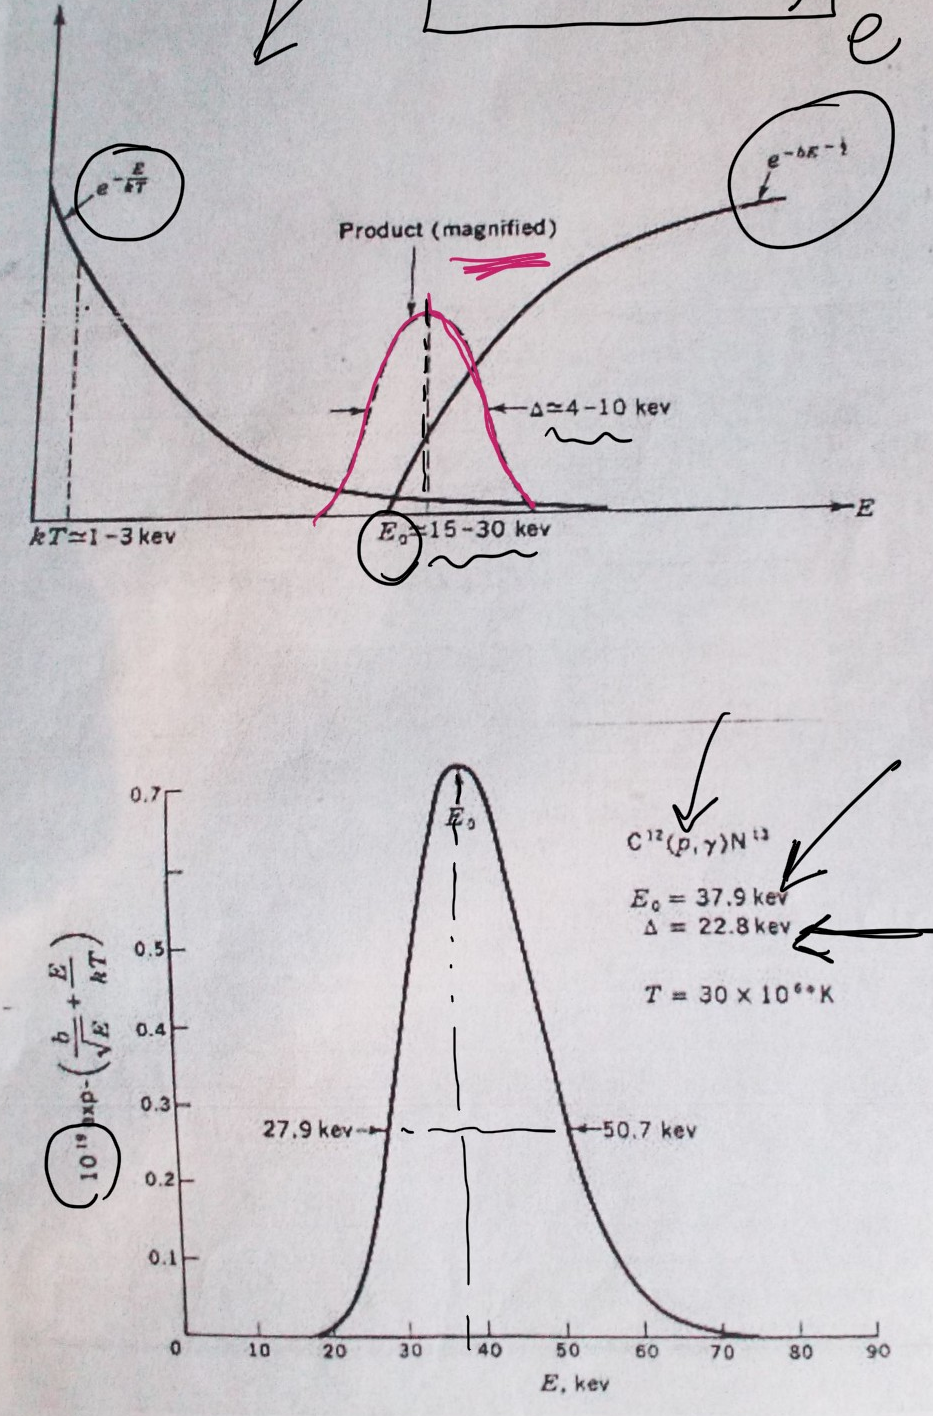
\includegraphics[scale=0.2]{Immagini/0324_gamow2.png}
    \caption{In alto l'andamento di $\exp{(-E/kT)}$, di $\exp{(-b/\sqrt{E})}$ e di $\exp{(-f(E))}$; in basso l'ingrandimento del picco di Gamow\index{picco di Gamow}.}
    \label{0324_picco}
\end{figure}
\noindent Dal momento che non conosciamo $S(E)$ per ogni $E$, cercheremo di sviluppare l'integrale e a tale scopo definiamo $\tau\equiv f(E_0)= 3E_0/kT$\footnote{$f(E_0)$ si calocola facilmente sostituendo $b=2E_0^{2/3}/kT$.} (nel Sole $\tau_{pp}\sim 14\gg 1$) e riscriviamo $f(E)$ come:
\begin{align*}
f(E) &= \PPc{\frac{E}{3E_0}\tau + \frac{b}{\sqrt{E}}\frac{kT}{3E_0} \tau} =\\
&= \tau \, \PPc{\frac{E}{3E_0} + \frac{2E_0^{3/2}}{kT \sqrt{E}}\frac{kT}{3E_0}} =\\
&= \tau \, \PPc{\frac{E}{3E_0} + \frac{2}{3}\sqrt{\frac{E_0}{E}}}\\
\text{Definiamo } x \text{ tale che } E&\equiv E_0 \ppc{1+\frac{2x}{\sqrt{\tau}}}\\
E-E_0 &= \frac{2x}{\sqrt{\tau}}E_0 = 2\sqrt{\frac{kTE_0}{3}}\,x \equiv \frac{\Delta}{2} x
\end{align*}
dove abbiamo definito $\Delta \equiv 4\sqrt{kTE_0/3}$ (per il Sole $\Delta_{pp}\sim 6.4$ keV)%che somiglia molto alla HWFH della Gaussiana
. Facciamo allora un'espansione\footnote{Si ricordi che $f'(E_0)=0$ e che $\tau/2E_0^2 = 8/\Delta^2$, per cui $f(x) = f(E_0) + ((E-E_0)/(\Delta/2))^2 + \dots$.} di $f(E)$ intorno a $E_0$, che in termini di $x$ è un'espansione intorno a $x=0$:
\begin{align*}
f(x) &= \tau \, \PPq{\frac{1}{3} \ppc{1+\frac{2x}{\sqrt{\tau}}} + \frac{2}{3} \frac{1}{\sqrt{\ppc{1+2x/\sqrt{\tau}}}}} \simeq\\
&\simeq \PPq{\frac{1}{3} \ppc{1+\frac{2x}{\sqrt{\tau}}} + \frac{2}{3} \PPc{1-\frac{x}{\sqrt{\tau}} +\frac{3}{2}\frac{x^2}{\tau} - \frac{5}{2} \frac{x^3}{\tau\sqrt{\tau}}+\frac{35}{8}\frac{x^4}{\tau^2}+ O(x^5)} } \simeq \\
&\simeq \tau  + x^2 - \frac{5}{3} \frac{x^3}{\sqrt{\tau}} + \frac{35}{12}\frac{x^4}{\tau}
\end{align*}
Sostituendo allora nell'integrale:
\begin{displaymath}
\begin{aligned}
\int_0^\infty S(E) \exp{(-f(E))}\,dE &\simeq \int_{-\sqrt{\tau}/2}^\infty dx\, S(x) \, \frac{2E_0}{\sqrt{\tau}} \: e^{-\tau} e^{-x^2} \, \underbrace{\exp{\ppc{\frac{5}{3} \frac{x^3}{\sqrt{\tau}} - \frac{35}{12}\frac{x^4}{\tau}}}}_\text{Parte non Gaussiana} \simeq \\
&\simeq  \int_{-\sqrt{\tau}/2}^\infty dx\, S(x) \, \frac{2E_0}{\sqrt{\tau}} \: e^{-\tau} e^{-x^2} \, \ppc{1+\frac{5}{3} \frac{x^3}{\sqrt{\tau}} - \frac{35}{12}\frac{x^4}{\tau} + \frac{25}{18} \frac{x^6}{\tau}}
\end{aligned}
\end{displaymath}
dove al primo passaggio abbiamo cambiato variabile $dE = dx\,2E_0/\sqrt{\tau}$ e successivamente sviluppato l'esponenziale al II ordine, trascurando i termini $O(x^7)$. Per procedere analiticamente con il calcolo sviluppiamo anche il fattore astrofisico\index{fattore astrofisico@fattore astrofisico $S(E)$} intorno a $E_0$: $S(E) = S(E_0) + (2xE_0/\sqrt{\tau})\,S'(E_0) + (2x^2E_0^2/\tau)\,S''(E_0)+\dots$; studiamo l'integrale dei vari ordini\footnote{Useremo principalmente che:
$$\int_{-\infty}^{+\infty} e^{-x^2} x^n = \Bigl \{ %
\begin{array}{ll}
    0 & n=2s+1 \\
    (2s-1)!!\:2^{-s} \: \sqrt{\pi} & n=2s
\end{array}%
$$%
Inoltre dal momento che $\tau$ è \vir{grande} (si guardi l'esempio di $\tau_{pp}$) si approssima nell'estremo dell'integrale $-\sqrt{\tau}\sim-\infty$ e poi si sfrutta la parità della funzione integranda.}:
\begin{displaymath}
\begin{aligned}
\text{Ordine 0}& \\
&S(E_0) \, \frac{2E_0}{\sqrt{\tau}}\,e^{-\tau} \int_{-\sqrt{\tau}/2}^\infty dx \:  e^{-x^2} \, \ppc{1+\frac{5}{3} \frac{x^3}{\sqrt{\tau}} - \frac{35}{12}\frac{x^4}{\tau} + \frac{25}{18} \frac{x^6}{\tau}}\simeq \\
\simeq\: &S(E_0) \, \frac{2E_0}{\sqrt{\tau}}\,e^{-\tau} \: 2\int_{0}^\infty dx \:  e^{-x^2} \, \ppc{1- \frac{35}{12}\frac{x^4}{\tau} + \frac{25}{18} \frac{x^6}{\tau}} = \\
= \:&\frac{2E_0}{\sqrt{\tau}}\,e^{-\tau} \,S(E_0) \,\sqrt{\pi}\; \ppc{1-\frac{5}{12}\frac{1}{\tau}} \\
\text{Ordine 1}& \\
&S'(E_0) \, \frac{4E_0^2}{\tau}\,e^{-\tau} \int_{-\sqrt{\tau}/2}^\infty dx \: x e^{-x^2} \, \ppc{1+\frac{5}{3} \frac{x^3}{\sqrt{\tau}} - \frac{35}{12}\frac{x^4}{\tau} + \frac{25}{18} \frac{x^6}{\tau}}\simeq \\
\simeq \:&S'(E_0) \, \frac{4E_0^2}{\tau}\,e^{-\tau} \:2\int_{0}^\infty dx \: x e^{-x^2} \, \frac{5}{3} \frac{x^3}{\sqrt{\tau}}= \\
=\:&\frac{5E_0^2}{\tau\sqrt{\tau}}\,e^{-\tau} \, S'(E_0) \,\sqrt{\pi} \\
\text{Ordine 2}& \\
&S''(E_0) \, \frac{4E_0^3}{\tau\sqrt{\tau}}\,e^{-\tau} \int_{-\sqrt{\tau}/2}^\infty dx \: x^2 e^{-x^2} \, \ppc{1+\frac{5}{3} \frac{x^3}{\sqrt{\tau}} - \frac{35}{12}\frac{x^4}{\tau} + \frac{25}{18} \frac{x^6}{\tau}}\simeq \\
\simeq\: &S''(E_0) \, \frac{4E_0^3}{\tau\sqrt{\tau}}\,e^{-\tau}\: 2 \int_{0}^\infty dx \: x^2 e^{-x^2} \, \ppc{1 \underbrace{- \frac{35}{12}\frac{x^4}{\tau} + \frac{25}{18} \frac{x^6}{\tau}}_{O(1/\tau^2)}}\simeq \\
\simeq \:&\frac{2E_0^3}{\tau\sqrt{\tau}}\,e^{-\tau}\,S''(E_0) \,\sqrt{\pi}
\end{aligned}
\end{displaymath}
Troviamo così per il \textit{reaction-rate}\index{reaction-rate@\textit{reaction-rate} $r$}:
\begin{displaymath}
\begin{aligned}
\mean{\sigma\,v } &=  \sqrt{\frac{8}{\pi\mu}} \ppc{\frac{1}{kT}}^{3/2} \frac{2E_0}{\sqrt{\tau}}e^{-\tau}\sqrt{\pi}\: \underbrace{ S(E_0) \PPq{1+\frac{1}{\tau} \PPc{\frac{5}{12} +\frac{5}{2} \frac{S'(E_0)}{S(E_0)}E_0 + \frac{S''(E_0)}{S(E_0)}E_0^2}} }_{S_{eff}} \equiv\\
&\equiv \sqrt{\frac{8}{\pi\mu}} \ppc{\frac{1}{kT}}^{3/2} \frac{2E_0}{\sqrt{\tau}}e^{-\tau}\sqrt{\pi}\; S_{eff} =\\
&= \frac{2^{7/2}}{3^{5/2}} \frac{\tau^2 e^{-\tau}}{b\sqrt{\mu}}\, S_{eff} \equiv\\
&\equiv K \frac{1}{AZ_1Z_2} \tau^2 e^{-\tau} \: S_{eff}
\end{aligned}
\end{displaymath}
dove abbiamo usato il fatto che\footnote{Si ricavano direttamente dalle definizioni di $b$ e di $\tau$.} $E_0 = (bkT/2)^{2/3}$ e $kT = 27\,b^2/4\tau^3$ e abbiamo definito il fattore astrofisico efficace $S_{eff}$\index{fattore astrofisico@fattore astrofisico $S(E)$!efficace@efficace $S_{eff}$} e la costante $K\simeq 7.2\cdot\ord{-19}$. Osserviamo che $\mean{\sigma\,v}$ dipende fortemente da $\tau$, ovvero dalla struttura della stella tramite $T$, e lo stesso vale per $S_{eff}$; per quanto riguarda quest'ultimo, facciamo uno sviluppo del fattore astrofisico e delle sue derivate in un intorno di $E=0$ fino all'ordine 2 in $S$\footnote{Per cui:%
\begin{displaymath}%
\begin{aligned}%
&S(E_0)   \simeq S(0) + S'(0) E_0 + \frac{1}{2} S''(0) E_0^2 \\ 
&S'(E_0)  \simeq  S'(0)  + S''(0) E_0 \\ 
&S''(E_0) \simeq  S''(0)
\end{aligned}%
\end{displaymath}%
}:
\begin{displaymath}
\begin{aligned}
S_{eff} &\simeq S(0)\, \ppc{1+\frac{5}{36}\frac{kT}{E_0}} +\\
&+ S'(0) E_0\, \ppc{1+\frac{35}{36}\frac{kT}{E_0}} +\\
&+ S''(0) E_0^2\, \frac{1}{2} \ppc{1+\frac{89}{36}\frac{kT}{E_0}}
\end{aligned}
\end{displaymath}
Questa espressione permette di trovare $S_{eff}$\index{fattore astrofisico@fattore astrofisico $S(E)$!efficace@efficace $S_{eff}$} indipendentemente dalla stella presa in considerazione, attraverso per esempio un fit polinomiale\footnote{Per \vir{calibrare} il fit ovviamente sono necessari degli input teorici che si ottengono dal \textit{match} tra la teoria e i dati sperimentali a energie più alte.} per $S(0)$, $S'(0)$ e $S''(0)$, tuttavia si perde l'informazione su $S(E_0)$ e gli errori per $E\sim0$ sono particolarmente rilevanti. 
Si ricordi che prima dell'esperimento LUNA\esperimento{LUNA} (i cui risultati sono riportati in turchese in Figura \ref{0315_astr}) non si avevano acquisizioni per basse energie tali da poter usare in un fit polinomiale, per cui la teoria era l'unica soluzione per esplorare tale \textit{range}.






